\documentclass{fennix}
\usepackage{graphicx}
\graphicspath{ {imagenes/} }

\begin{document}
	\title{Introducción al ASM en GNU/Linux x86 \& x86-64}
	\author{Tryger \& b10s\_0v3rr1d3}
	\date{2015-09-03 -- 2015-09-03}
	\maketitle
\begin{resumen}
	0x01 - Registros generales y básicos.
\end{resumen}

\begin{requisitos}
	\begin{itemize}
		\item OS GNU/Linux - Distribución independiente 
		\item Ensamblador NASM. 
		\item Debugger GDB (por defecto en gnu/linux). 
	\end{itemize}
\end{requisitos}

\section{Introducción}
Bienvenido a la primera parte e introducción de este nuevo curso para aprender lenguaje ensamblador (asm de ahora en adelante).\\
\\
Este curso será escrito por tryger y yo mismo (b10s\_0v3rr1d3) y trataremos en el, desde la parte mas básica como sera todo este bloque inicial (introducción, memoria, tipos de datos y variables, stack, etc....), un bloque intermedio para las operaciones e instrucciones (aritmeticológicas, jumps, etc...) y por último un bloque mas avanzado donde ya daremos aspectos mucho mas complejos.\\
\\
Comentar también que procuraremos hacer este curso lo mas dinámico y practico posible, que aunque la teoría nunca viene mal no todo es teoría ;)\\
\\
Hay que decir que la sintaxis que se usara en este curso es intel (que no es la única existente, pero es la que usaremos).
El compilador que usaremos durante este curso sera el 'nasm' y entre los debuggers que podremos utilizar, de base (y que por norma general suele estar por defecto en los OS instalado) es el GDB (Gnu debugger) [mas info].
Decir que en este curso inicialmente daremos uso de dicho debugger, pero también en un futuro mostremos el uso de otros como lo es 'radare' por ejemplo.\\
\\
Una vez dicho esto y para no alargar la introducción, daremos comienzo con los distintos tipos de registros que podemos encontrar en nuestra CPU que son básicos para empezar. 

\newpage
\section{Registros de propósito general}
Si en algún momento has usado algún debugger o parecido, habrás visto en mas de una ocasión palabras como 'eax', 'ebx', etc...\\
Estos son los principales registros que tiene la CPU y que pueden dividirse como podrás observar en distintos tamaños:\\
\\
\textbf{EAX}
\begin{figure}[h]
	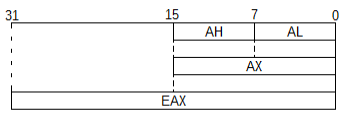
\includegraphics{eax}
	\centering
	\caption{\underline{Acumulador}, se suele usar para guardar datos, los operadores en una operación, resultados de las mismas, etc...}
\end{figure}
\\
\textbf{EBX}
\begin{figure}[h]
	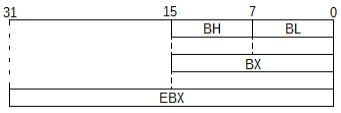
\includegraphics{ebx}
	\centering
	\caption{Se suele usar como un puntero hacia los datos}
\end{figure}
\\
\textbf{ECX}
\begin{figure}[h]
	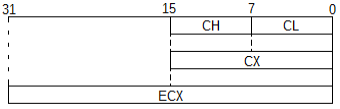
\includegraphics{ecx}
	\centering
	\caption{Registro para contadores (loops)}
\end{figure}
\newpage
\textbf{EDX}
\begin{figure}[h]
	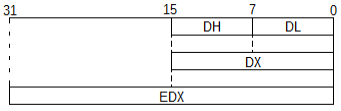
\includegraphics{edx}
	\centering
	\caption{Registro para datos, suele usarse como puntero para I/O}
\end{figure}
\\
Todos los anteriores pueden ser divididos hasta un tamaño de 8 bits como se puede ver perfectamente en las imágenes y los nombres que tienen asignados a esos mismos tamaños (como podeis ver, los mas pequeños tienen una 'H' o una 'L' si se refieren a los bits mas altos o mas bajos de dentro del registro (dentro de la división de 16 bits).
Los siguientes de la lista son también de propósito general pero unicamente pueden dividirse hasta bloques de 16 bits:
\textbf{ESP}
\begin{figure}[h]
	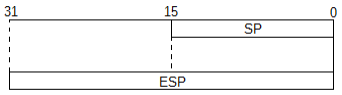
\includegraphics{esp}
	\centering
	\caption{\underline{Stack pointer}, puntero que nos indica la dirección actual del 'stack'}
\end{figure}
\\
\textbf{EBP}
\begin{figure}[h]
	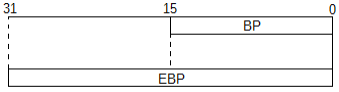
\includegraphics{ebp}
	\centering
	\caption{Parecido al anterior pero en este caso no apunta a la dirección actual sino que apunta a la base de dicho stack}
\end{figure}
\newpage
\textbf{ESI/EDI}
\begin{figure}[h]
	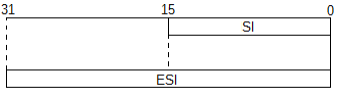
\includegraphics{esi}
	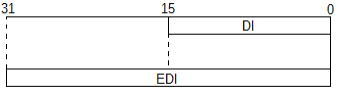
\includegraphics{edi}
	\centering
	\caption{Punteros para el trabajo con la memoria (veremos esto mas adelante en el curso)}
\end{figure}
\\
Como podéis ver, debajo mismo de la división de tamaños tenéis también el uso común que se les suele dar a cada uno de los mismos registros que se han comentado.

\newpage
\section{Registros de segmento}
Estos registros pueden depender en parte de lo que se llama 'memory mode' (resumido 'la forma de direccionamiento de la memoria') [esto se vera mas detallado en el apartado de la memoria de este curso].
Todos ellos son del mismo tamaño, 16 bits [0-15] y no se subdividen como los otros registros que hemos visto.\\
\\
Los nombres son los siguientes y el nombre que se les suele asignar:\\
\\
\textbf{Code Segment} [CS]\\
\\
\textbf{Data Segment} [DS]\\
\\
\textbf{Stack Segment} [SS]\\
\\
\textbf{Data Segment} [ES] [FS] [GS]\\
\\
Como he comentado, veremos muchos mas detalles de estos registros en siguientes capítulos donde se podrán ver y entender mejor de forma práctica.\\

\section{Registro EFLAGS}
Es un registro de 32 bits [0-31] que nos permite ver distintos estados de nuestra CPU según las operaciones que hemos estado haciendo anteriormente.\\
\\
Este registro tiene bastante importancia (como veréis en el apartado de los saltos [jumps] por ejemplo) ya que es el registro que indica mediante la activación de los bits de cada una de las posiciones un tipo de significado u otro.\\
Podemos poner un ejemplo haciendo una simple operación matemática para ver el porque de algunos de los flags que tenemos:\\
\\
Como todos sabemos, la siguiente operación → [8 + 4], da como resultado 12 (sorprendente eh?).\\
Bien esto que nos parece tan simple y obvio, podemos ver que si lo 'analizamos', tenemos lo que se llama 1 acarreo (que imagino todos sabemos lo que es).\\
Pues en nuestra CPU, nos marcaría el 'carry flag' (bit de acarreo) para indicar que la operación ha tenido un 'desbordamiento' ya que ha pasado de ocupar un dígito (los sumandos) a dos dígitos (el resultado).\\
\\
Otros ejemplo, el 'Zero flag' que (como imaginaras) nos indica si la operación ha dado como resultado 0.\\

\newpage
\section{Registro EIP}
El tamaño de este registro es de 32 bits [0-31] y es uno de los registros mas importantes como ahora mismo podrás ver.\\
Este registro es lo que se podría decir 'Instruction Pointer' y que nos indica (mediante la dirección de memoria que esta apuntando) cual es la siguiente instrucción que nuestra CPU va a ejecutar.\\
Que importancia tiene este registro te preguntaras?, pues simple (y como deberías poder deducir) imaginate lo que pasa si en lugar de apuntar en la dirección de memoria a la que tiene que apuntar en su normal funcionamiento este registro apunta a una dirección de memoria que tu mismo has 'manipulado' dicho puntero para que posteriormente la CPU ejecute las siguientes instrucciones que nos interesan.\\
\\
Básicamente este registro suele llamarse el diamante del shellcoding, exploits, etc....\\

\newpage
\section{Unidad de coma flotante (FPU) x87}
Bien en el siguiente apartado comentaremos varios aspectos de la unidad de coma flotante que actualmente disponen las CPU.\\
El x87 es lo que se podría llamar el 'grupo' dentro de las instrucciones de la arquitectura x86 especializada en las tareas referidas a las operaciones en coma flotante.\\
Permiten trabajar con dicho tipo de operaciones y valores con (inicialmente) distintos niveles de precisión a nivel binario, ya sea simple precisión, doble precisión o (como suele estar por defecto mayormente) la precisión de 80 bits (tamaño de los registros que en breve comentaremos).\\
Los registros de base de esta unidad son 8 en forma de 'stack' (pila) y que usan la siguiente nomenclatura [ST(0) – ST(7)]\\
Dichos registros tienen lo que podríamos decir un 'truco' a la hora de acceder a ellos, ya que se utiliza un sistema mediante desplazamientos relativos al 'top' (tope) del 'stack' de los mismos (esto incluye el hecho del uso de 'push \& pop' para trabajar con dichos registros (lo que seria apilar y desapilar).\\
\\
A continuación nos encontramos también con las distintas extensiones 'agrupadas' dentro de lo que se llamaría SIMD (Single Instruction Multiple Data).
Estas extensiones son por ejemplo, MMX, SSE, SSE2, SSE3...\\
\\
Las instrucciones de MMX trabajan en lo que podriamos ver como 'subregistros' dentro de los registros que hemos visto anteriormente (ST) ya que usan los primeros 64 bits de los 80 que disponen los registros ST.\\
Evidentemente como te puedes imaginar, los nombres de dichos registros usan una nomenclatura similar a los anteriores; MM0 – MM7\\
De estos hay algunos detalles que hay que tener presentes.\\
Por una parte a diferencia de los anteriores que hemos visto, si permiten el acceso directo a los mismos (si recuerdas lo comentado hace un momento, los registros ST tenian sus 'trucos' a la hora de acceder a ellos).\\
Y por otro lado el hecho que estos registros pueden afectar y/o ser afectados en operaciones hechas a los registros ST (como bien puedes imaginar, si resulta que son unos 'subregistros' de ellos, a la que modificar una cosa que afecte los primeros bits de ellos, afectas a los 2.\\
\\
Por otra parte la extension SSE nos brinda un nuevo conjunto de instrucciones y tambien un grupo de registros que comentaremos, no sin antes comentar que este tipo de instrucciones suelen ser mas utilizadas para el proceso de graficos, senales digitales, etc...\\
Los registros tambien usan una nomenclatura bastante sencilla similar a los anteriores; [XMM0 – XMM 7]\\
Otra diferencia a comentar con los distintos registros que hemos visto, es el tamano que disponen estos, nada menos que 128 bits [0-127].\\
Comentado toda esta ultima parte (y no hacerla mucho mas extensa porque podría alargarse mucho por la cantidad de detalles que hay), dejaremos esta primera parte de la introducción al ASM aquí.\\
\\
Hemos comentado los distintos registros de base y principales que suelen disponer la mayoría de CPU (ya que en algunos casos puede variar según si la CPU tiene ciertas extensiones habilitadas o no).\\
\\
Hasta aquí la primera parte de nuestro curso.\\
Nos leemos ;)

\newpage
\section{[Anexo I] Registros x86-64}
En este anexo, comentaremos los distintos registros que nos encontraremos en caso que trabajemos en un entorno de 64 bits.\\
Hay que decir que en esta ocasión no iremos tanto al detalle ya que realmente, no es muy difícil ver las diferencias entre 32 bits y 64 bits y en algunos aspectos es aplicar lo que llamaríamos 'código mnemotécnico'.\\
\\
En la siguiente imagen, podemos ver un resumen general de los distintos registros que nos podemos encontrar:\\
\begin{figure}[h]
	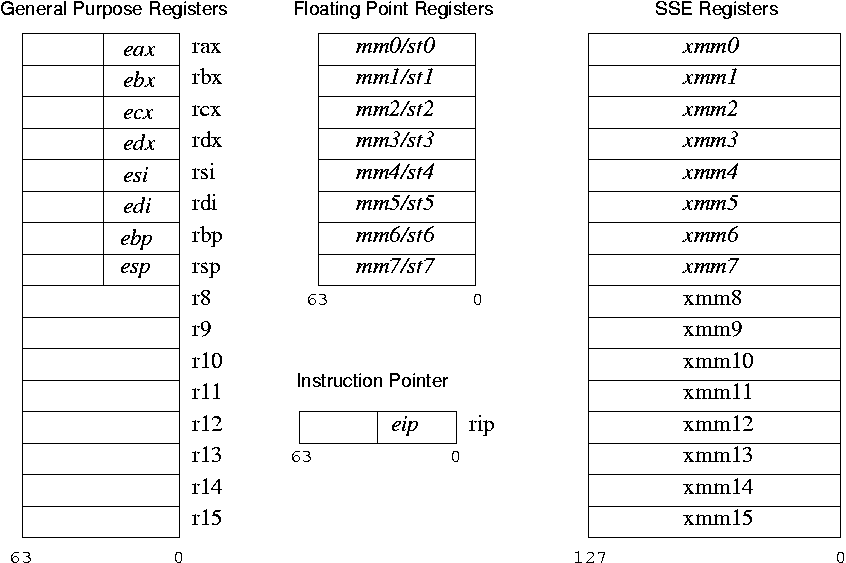
\includegraphics[width=\textwidth]{x86-64}
	\centering
\end{figure}
\\
Como puedes observar en la anterior tabla, los distintos registros a excepción de los SSE, han duplicado el tamaño (hay que comentar el hecho que los SSE pueden ser de distinto tamaño si nuestra CPU tiene el juego de instrucciones AVX que pasarían a 256, etc... (esto ultimo lo veremos mas adelante sin ningún problema, por el momento es mas un detalle)).\\
\\
En los registros de propósito general, hay una forma fácil de verlos y acordarse, simplemente como podéis ver en sus nombres, substituir la 'e' por una 'r' y tenemos disponibles 8 registros mas, que son los últimos que aparecen [R8 – R15].\\
\\
El EIP que vimos, también nos dobla el tamaño y como hemos comentado hace un momento, el nombre substituye la 'e' por la 'r'.\\
\\
Aunque no aparece en la imagen, los EFLAGS también han crecido a 64 bits de tamaño y usan la misma formula para el nombre (pasa de EFLAGS a RFLAGS).\\
\\
Los registros ST y MM se quedan como veis iguales, por lo que no tiene mucho misterio volver a repetirlo.\\
\\
Los últimos que comentamos de la extensión SSE, los registros XMM, pasamos de tener 8 a tener 16 y como podéis ver no tiene mucha mas complicación ya que tienen los mismos nombres [XMM0 – XMM15].\\
Deberíamos tener en cuenta por ejemplo, que en el detalle que comente del AVX, los nombres de dichos registros se verían afectados y pasarían de XMM a YMM, el tamaño 256 e igualmente a 16 registros.... (pero eso ya es un detalle que comentaríamos mas adelante)\\
\\
Luego otro detalle que seguramente se puede ver es que en el caso de los registros de segmento que comentamos, en 64 se suelen usar unicamente los 2 últimos (FS y GS).\\
Esto se debe básicamente a que no suelen usarse mucho dichos registros por no decir que no se usan (podríamos entrar mas en detalle ya que por ejemplo una de las razones es que con direcciones de memoria de 64 bits puedes direccionar mucha mas memoria de la que normalmente tendrás en tu PC y se hace innecesario su uso, pero tampoco hace falta dar mucha mas vuelta)\\
\\
Bien, comentados estos detalles mas generales entre 32 y 64 bits, damos fin al pequeño anexo para los registros en 64 bits.\\
\\
En breve pondremos un pequeño documento adicional a esta primera parte introductoria con ejemplos y muestras para hacerlo mas visible y mas fácil de entender para todos aquellos que tengáis dudas o que os sea mas difícil verlo ;)\\
\\
Nos leemos, saludos :P

\begin{colabs}
	Tryger: mail1
	
	b10s\_0v3rr1d3: b10s\_0v3rr1d3\@c0d3\-l4bs.net
\end{colabs}

\end{document}
